\section{Meta-Heuristiken}
\subsection{Hill-Climbing \skript{2}}
  Konvergiert meist in lokales Optimum, Konvergenz sehr langsam., Wahl eines Zufallsschritts ist schwierig. Zielfunktion muss oft berechnet werden.
  
  Algorithmus, um Zielfunktion $f(\vec{x})$zu maximieren:
  \begin{enumerate}
    \item Start: Wahl von $\vec{x}^{alt}$
    \item Neue Wahl $\vec{x}^{neu}$ "`in der Nähe"' von $\vec{x}^{alt}$ {\tiny (Das war die komische Bitschieberei in der Vorlesung)}
    \item Wenn $f(\vec{x}^{neu}) \geq f(\vec{x}^{alt})$, setze $\vec{x}^{alt} = \vec{x}^{neu}$ und gehe zu Schritt 2
  \end{enumerate}
  
 

\subsection{Tabu-Search \skript{3}}
  Grundidee: Keine / möglichst wenige Schritte, welche die Wirkung früherer Schritte rückgängig machen.
  
  Etwas schnellere Konvergenz ggn. Hill-Climbing, allerdings aufwendiges Mitführen und Aktualisieren der Tabu-Liste sowie Schwierigkeit, um Länge der Tabu-Liste zu finden. Zielfunktion muss oft berechnet werden.
  
  Algorithmus, um Zielfunktion $f(\vec{x})$zu maximieren:
  \begin{enumerate}
    \item Start: Wahl von $\vec{x}^{alt}$
    \item Neue Wahl $\vec{x}^{neu}$ "`in der Nähe"' von $\vec{x}^{alt}$, welche mit einem erlaubten Schritt $m_i \notin T$ eine möglichst gute Verbesserung (oder geringste Verschlechterung bringt).
    \item Einfügen des komplementären Schritts $\bar{m}_i$ in Tabu-Liste $T$.
    \item Schritte 2 und 3 wiederholen, bis vorgegebenes Abbruchkriterium erreicht ist.
  \end{enumerate}

\subsection{Simulated Annealing \skript{5}}
  Grundidee: Gegenüber dem Tabu-Search wird eine Verschlechterung der Lösung mit einer gewissen Wahrscheinlichkeit akzeptiert. So kann ein lokales Optimum wieder verlassen werden.
  
  \begin{enumerate}
    \item Start: Wahl von $\vec{x}^{alt}$
    \item Neue Wahl $\vec{x}^{neu}$ "`in der Nähe"' von $\vec{x}^{alt}$
    \item Wenn $f(\vec{x}^{neu}) \geq f(\vec{x}^{alt})$ oder mit einer Wahrscheinlichkeit von $p = e^{\frac{-\Delta E}{T}}$, setze $\vec{x}^{alt} = \vec{x}^{neu}$.
    \item Schritte 2 und 3 wiederholen, bis vorgegebenes Abbruchkriterium erreicht ist.
  \end{enumerate}
  
  Wahl der Parameter:
  \begin{itemize}
    \item $\Delta E$: Wenn Minimum: $\Delta E = f(\vec{x}^{neu}) - f(\vec{x}^{alt})$; wenn Maximum: $\Delta E = f(\vec{x}^{alt}) - f(\vec{x}^{neu})$
    \item Veränderung der Temperatur $T(i)$ (Kühlschema): Konstant, arithmetisch (bei jedem Schritt wird um gleichen Betrag verkleinert), geometrisch (bei jedem Schritt wird um gleichen Faktor verkleinert), stufenweise (diskrete Sprünge)
    \item Anfangstemperatur $T(0)$: Z.B. mittlere Änderung der Zielfunktion über einige zufällig gewählte Schritte.
  \end{itemize}
  

\subsection{Genetische Algorithmen (GA) \skript{8}}
  \begin{minipage}{12cm}
    Löst alle Klassen von schwierigen Optimierungsproblemen: Parameteroptimierungen, kombinatorische Probleme (e.g. Travelling Salesman), Subset-Selektion (Stichwort Data-Mining).
  
    Grundprinzip: Durch \em Selektion \em (Fitness/objective function), \em Rekombination \em (Kombination des genetischen Materials der Eltern) und \em Mutation \em (Veränderung der Erbinformation) können Funktionen optimiert werden. Dabei wird iterativ von einer "`alten"' Population durch verschiedene Operationen eine neue Population generiert, welche im Normalfall gleich gross sein soll.\\
    
    Beispiel eines GA-Modells:\\
    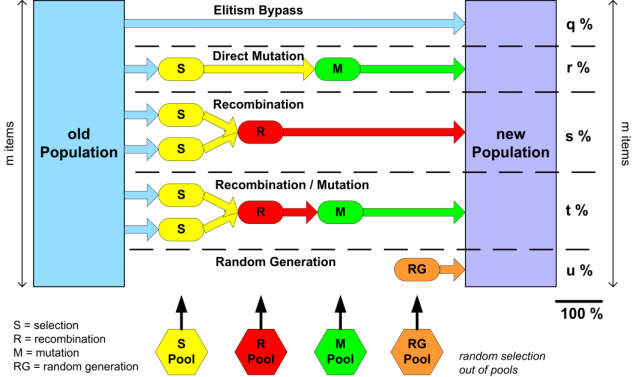
\includegraphics[width=12cm]{./Content/MetaHeuristics/GeneticAlgorithms_Model}
  \end{minipage}
  \begin{minipage}{7cm}
   \begin{flushright}
    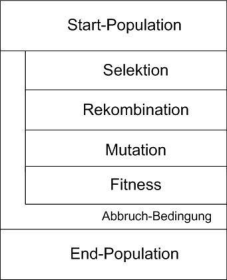
\includegraphics[width=6cm]{./Content/MetaHeuristics/GeneticAlgorithms_Principle}
   \end{flushright}
    
    \subsubsection{Codierung der Parameter \skript{11}}
      Am besten werden die Parameter \em Gray\em -codiert, damit Mutationen nicht zu sehr ins Gewicht fallen:
      
      \begin{center}
        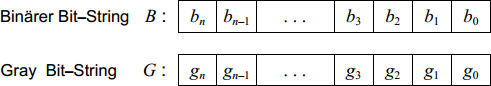
\includegraphics[width=7cm]{./Content/MetaHeuristics/GeneticAlgorithms_Gray}
      \end{center}
      $$g_j = \begin{cases}
        b_n                & j=n\\
        b_{j+1} \oplus b_j & j < n
        \end{cases} \qquad \qquad 
      b_j = \sum \limits_{k=n}^j \oplus g_k$$
  \end{minipage}
  
\subsubsection{Selektion \skript{15}}
  Probabilistische (Zufallsprinzip, z.B. \em Roulette-Wheel\em ) oder deterministische (nach Fitnesswerten, z.B. nur die besten; z.B. \em Binäre Wettkampfselektion\em ) Selektion. Problem bei beiden: Die besten Gene können verloren gehen, deshalb werden meist das beste oder die besten Individuen übernommen.
  
\subsubsection{Rekombination \skript{16}}
  \begin{tabularx}{\textwidth}{p{9cm} p{9cm}}
    \em One-Point Crossover\em : Der "`Chromosomen"'-String wird an zufälliger Stelle getrennt und neu rekombiniert: 
      & \em Two-Point Crossover\em : Der "`Chromosomen"'-String wird an zwei zufälligen Stellen getrennt und neu rekombiniert: \\
    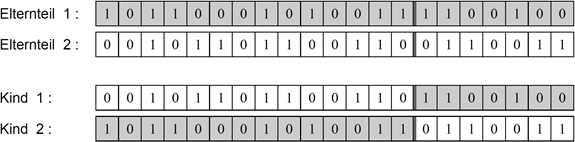
\includegraphics[width=8cm]{./Content/MetaHeuristics/GeneticAlgorithms_OnePointCrossover}
      & 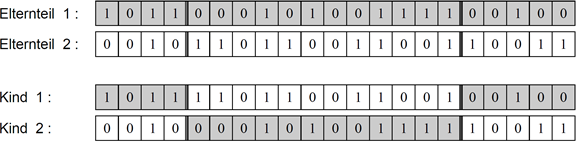
\includegraphics[width=8cm]{./Content/MetaHeuristics/GeneticAlgorithms_TwoPointCrossover} \\ \\
    \em $k$-Point Crossover\em : Verallgemeinerung von One-/Two-Point Crossover.
      & \em Uniform Crossover\em : $k$-Point Crossover mit Grenzwert $k \rightarrow n$, hier wird also jedes Bit zufällig kombiniert.
  \end{tabularx}
   
  
\subsubsection{Mutation \skript{18}}
  \begin{minipage}{8cm}
    \begin{itemize}
      \item \em Bit-Flip-Mutation\em : Zufällig ausgewählte Bits werden invertiert, wobei dies mit (kleiner) Wahrscheinlichkeit (Mutationsrate) geschieht.
      \item \em Positionsmutation\em : Bits oder ganze Bitstrings können an verschiedenen Positionen ausgetauscht werden.
      \item \em Inversion\em : Bits können auch invertiert werden (Auswahl durch Zufall). \todo{RK: check, komische Erklärung im Skript}
    \end{itemize}
  \end{minipage}
  \begin{minipage}{11cm}
    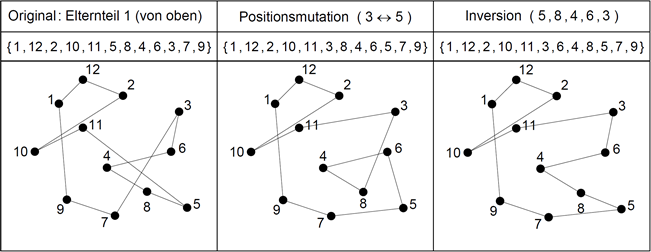
\includegraphics[width=11cm]{./Content/MetaHeuristics/GeneticAlgorithms_Mutation}
  \end{minipage}
  
 \subsubsection{Ersetzungsschemata \skript{19}}
   Was passiert mit der alten Population? 
   
   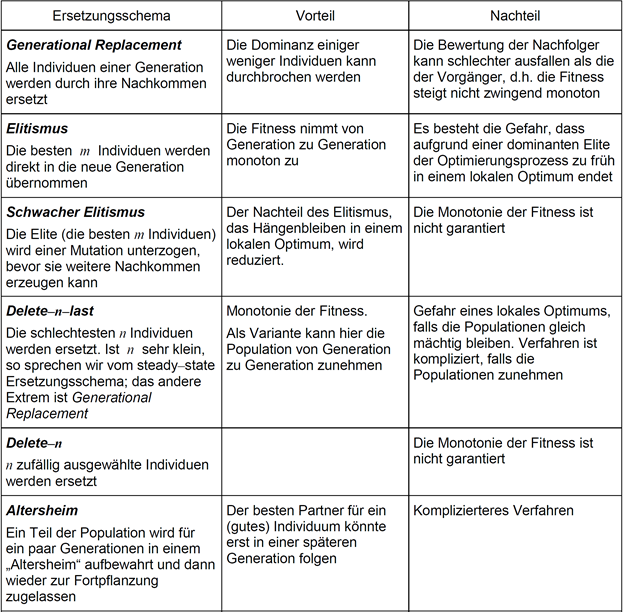
\includegraphics[width=12cm]{./Content/MetaHeuristics/GeneticAlgorithms_Replacements}
   
   
 \subsection{Ant Colony Optimization \skript{21}}
   Ameisen folgen intensiven Pheromon-Spuren, da dort die Chance auf Futter zu treffen gross ist. Diese Idee wird bei ACO aufgenommen. Mit einer Wahrscheinlichkeit $P(x_{ij})$ wird ein möglicher Pfad $ij$ in die neue Generation übernommen. Zusätzlich wird meist auch ein "`Elite-Bypass"' mit Schwellwert $Q$ implementiert:
   $$P(x_{ij}) = 
   \begin{cases}
     \text{if } z < Q = 
     \begin{cases}
       1 & \text{if } j = \arg \max\limits_{k \in \mathbf{W}_i}[\tau_{ik}^\alpha \eta_{ik}^\beta] \\
       0 & \text{else}
     \end{cases} \\
     \text{if } z \geq Q
     \begin{cases}
       \dfrac{\tau_{ij^\alpha \eta_{ij}^\beta}}{\sum\limits_{j \in \mathbf{W}_i} \tau_{ij^\alpha \eta_{ij}^\beta}}  & \text{if }j \in \mathbf{W}_i\\
       0 & \text{else}
     \end{cases}
   \end{cases}$$
   mit $\eta_{ij}$ als heuristischer Information (z.B. $\eta_{ij} = \frac{1}{d_{ij}}$ beim TSP)
 \lstinputlisting[language=Java]{./Content/MetaHeuristics/ACO.java}
 
 \subsection{Particle Swarm Optimization \skript{23}}
 
 